\documentclass[main.tex]{subfiles}

\begin{document}

\chapter{Methodology}

\section{Spline evaluation}
A B-spline function is a combination of flexible bands that is controlled by a number of points that are called control points, creating smooth curves. These functions enable the creation and management of complex shapes and surfaces using a number of points. B-spline function and Bézier functions are applied extensively in shape optimization methods.[4]

A B-spline of order n { n} n is a piecewise polynomial function of degree n − 1 { n-1} n-1 in a variable x { x} x. It is defined over 1 + n { 1+n} { 1+n} locations t j { $t_{j}$} { $t_{j}$}, called knots or breakpoints, which must be in non-descending order t j ≤ t j + 1 { $t_{j}\leq t_{j+1}$} { $t_{j}\leq t_{j+1}$}. The B-spline contributes only in the range between the first and last of these knots and is zero elsewhere. If each knot is separated by the same distance h { h} h (where h = t j + 1 − t j { $h=t_{j+1}-t_{j}$} {$h=t_{j+1}-t_{j}$}) from its predecessor, the knot vector and the corresponding B-splines are called 'uniform' (see cardinal B-spline below).

For each finite knot interval where it is non-zero, a B-spline is a polynomial of degree n − 1 { n-1} n-1. A B-spline is a continuous function at the knots.[note 1] When all knots belonging to the B-spline are distinct, its derivatives are also continuous up to the derivative of degree n − 2 { n-2} n-2. If the knots are coincident at a given value of x { x} x, the continuity of derivative order is reduced by 1 for each additional coincident knot. B-splines may share a subset of their knots, but two B-splines defined over exactly the same knots are identical. In other words, a B-spline is uniquely defined by its knots.

One distinguishes internal knots and end points. Internal knots cover the x { x} x-domain one is interested in. Since a single B-spline already extends over 1 + n { 1+n} { 1+n} knots, it follows that the internal knots need to be extended with n − 1 { n-1} n-1 end points on each side, to give full support to the first and last B-spline which affect the internal knot intervals. The values of the endpoints do not matter, usually the first or last internal knot is just repeated.\\

de Boor's algorithm, an efficient and numerically stable scheme to evaluate a spline curve S ( x ) { \mathbf {S} (x)} {\mathbf {S} (x)} at position x { x} x.

The usefulness of B-splines lies in the fact that any spline function of order n { n} n on a given set of knots can be expressed as a linear combination of B-splines: 
\begin{equation}
    S(t) = \sum_{i}^{n-1}C_{i}\phi_{}^{k}(t)
\end{equation}
\section{Segmentation Backbone}
\section{Preprocessing}
\subsection{Contour extraction}
Linear interpolation of the contours points to be of a single length for computational purpouses.
\subsection{Object probabilities}
We compute the object probabilities by applying a normalized euclidean distance for each instance
\subsection{Overlap probabilities}
Overlap probability equal 1 if two object overlap otherwise 0, this will be usefull to provide a posteriori proposal probability
\section{Postprocessing}
\subsection{Non Maximum Suppresion}
Each pixel of the output image correspond to an object instance, therefore detecting the same object multiple times, in order to get a single prediction for each object We use typical non maximum suppression. where we keep objects whith the highest probabilities and suppress the instances that have Intersection Over Union bigger than a certain threshold.

\subsection{Matching instances with the Ground truth}
Once we have a final objects predictions, we match it with the ground truth objects, we define True Positives as objects having IoU over some threshold, False Negative objects in ground truth that have no correspondance, False positive Objects in prediction that have no correspondance in the ground truth.
\section{Metrics}
\subsection{Distance Between two instances}
We modelise the problem as a binary assignment problem, where each pixel from the first contour has a single unique matching from the second.\\

The linear sum assignment problem is also known as minimum weight matching in bipartite graphs. A problem instance is described by a matrix C, where each $C_{ij}$ is the cost of matching vertex i of the first partite set (a “worker”) and vertex j of the second set (a “job”). The goal is to find a complete assignment of workers to jobs of minimal cost.\\

Formally, let X be a boolean matrix where 
\begin{equation}
    X_{i,j}=\left\{
                \begin{array}{ll}
                  1 \quad\quad \textit{if row i is assigned to column j}\\
                  0 \quad\quad else
                \end{array}
              \right.
\end{equation}
Then the optimal assignment has cost
\begin{equation}
    \min \sum_i \sum_j C_{ij}X_{ij}
\end{equation}

Each row is assignment to at most one column, and each column to at most one row. The method used is the Hungarian algorithm, also known as the Munkres or Kuhn-Munkres algorithm.

\begin{figure}
    \centering
    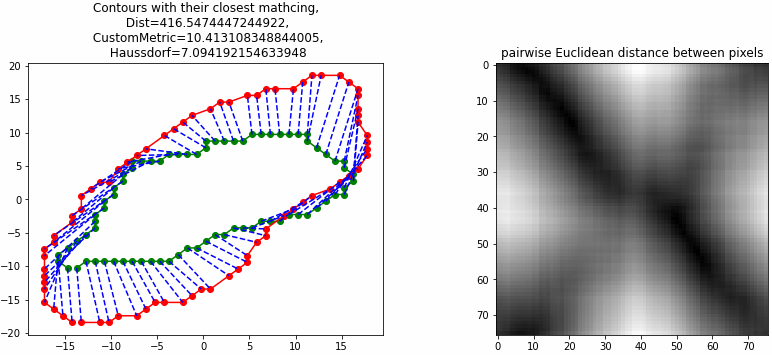
\includegraphics[width=16cm]{images/contourMatching.PNG}
    \caption{Exemple of the matching between pixels from the first contour ans the second contour}
\end{figure}
\section{Loss formulation}
% \begin{equation}
    
% \end{equation}
\section{Evaluation}
We use K-Fols cross validation 
\section{3D adaptation}
We solve the binary association problem between slices of the 3d image
\end{document}


